\begin{center}
{\Large {\bf Figures}}
\vspace{1.5cm}
\end{center}

\begin{figure}[h!]
\begin{center}
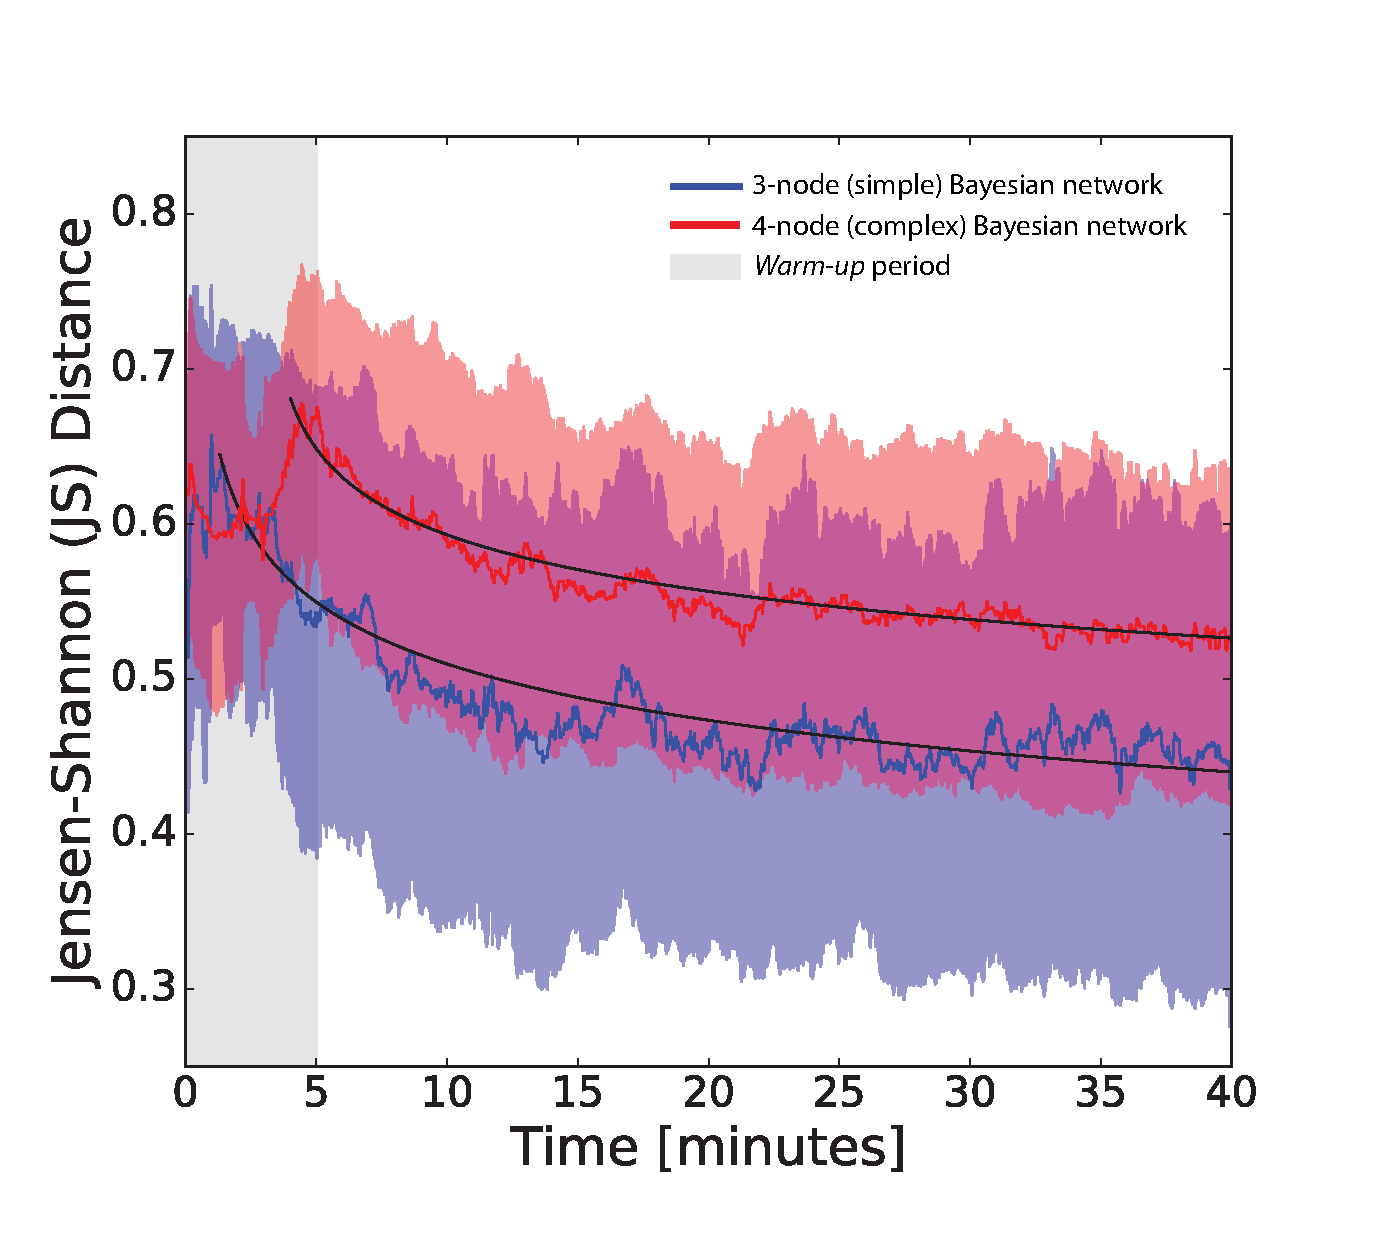
\includegraphics[width=12cm]{figures/decay_simple_complex.eps}
\caption{\footnotesize Decay of the Jensen-Shannon (JS) Distance (\ref{JS-distance}) between models proposed by participants and the true model over time for the 3-node (simple) and 4-node (complex) Bayesian network treatments (resp. in blue and red). The colored areas show the standard deviation. The decays are averaged (mean) over all participants for each treatment. Both treatments follow similar extremely slow power law decay (\ref{power_law_decay}), yet with different exponents: $\alpha = 0.1$ ($p < 0.001$, $R = -0.92$) for the simple Bayesian network treatment and $\alpha = 0.07$ ($p < 0.001$, $R = -0.94$) for the complex Bayesian treatment. The grey area on the left shows the 5-minute {\it warm up} period during which participants get used to the interface. In both treatments, participants elaborate initial Bayesian Net models with $JSD \approx 0.6$, and there is a phase associated with counter-performance (during which the JS Distance increases). This phase is however much shorter for the simple Bayes Net (peak at $t \approx1$ minute) compared to the complex Bayes Net (peak at $t \approx 4.5$ minutes) after which the JS-distance actually starts to decay.}
\label{fig:decay}
\end{center}
\end{figure}

\begin{figure}[h!]
\begin{center}
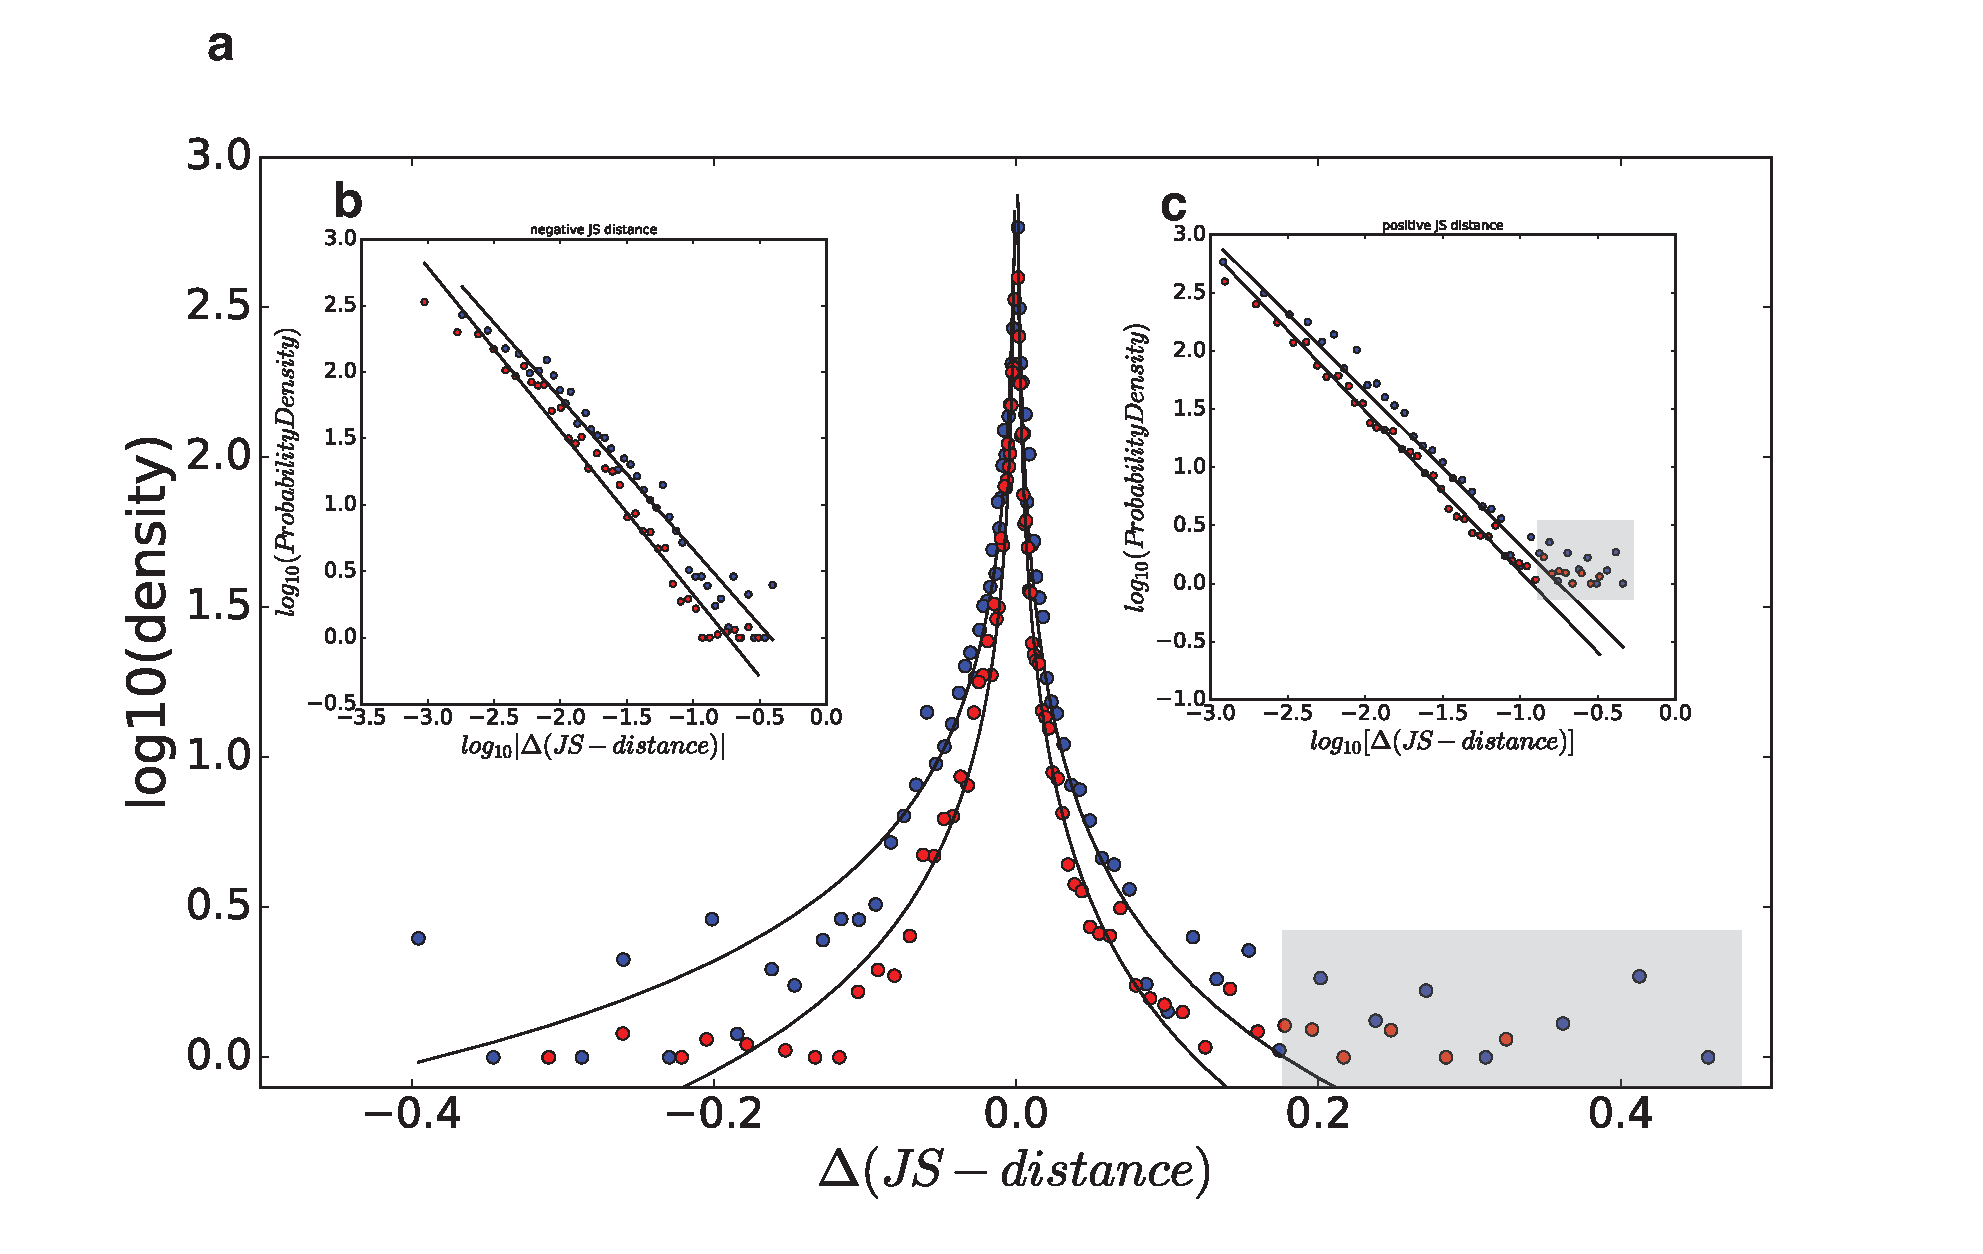
\includegraphics[width=15cm]{figures/pdf_JSD.eps}
\caption{{\bf a.} Probability density function (un-normalized) of $\Delta(JS-distance)$ ($\Delta JSD$) between 2 consecutive changes (jump sizes). The negative $\Delta(JS-distance) < 0$ stands for improvement (i.e., the goal is to reduce the $JS-distance$). On the contrary, the $\Delta(JS-distance) >  0$ happens when a participant comes up with a BayesNet model which is further from the true model, compared to the previous attempt. The distribution is heavy-tailed on both sides (c.f., {\bf b.} and {\bf c.}), almost power law tail, yet with some particularities: For $\Delta JSD < 0$, the probability density function may be a {\bf log-normal}. For $\Delta JSD > 0$, an extra ``outliers" regime is present (grey shade rectangle). Also, $\Delta JSD > 0$ is more heavy-tailed compared to $\Delta JSD < 0$ (see Table \ref{pwlaw_fits}). The {\it simple} and {\it complex} treatments (resp. blue and red dots) look similar, yet with sligtly different exponents (see again Table \ref{pwlaw_fits}). Interestingly, the median in both simple and complex cases is very close to zero [$median(pdf) < 0.001$], which means that on average, after a change was made to a model the model is only a slight improvement over the old.}
\label{fig:jump_sizes}
\end{center}
\end{figure}


\begin{figure}[h!]
\begin{center}
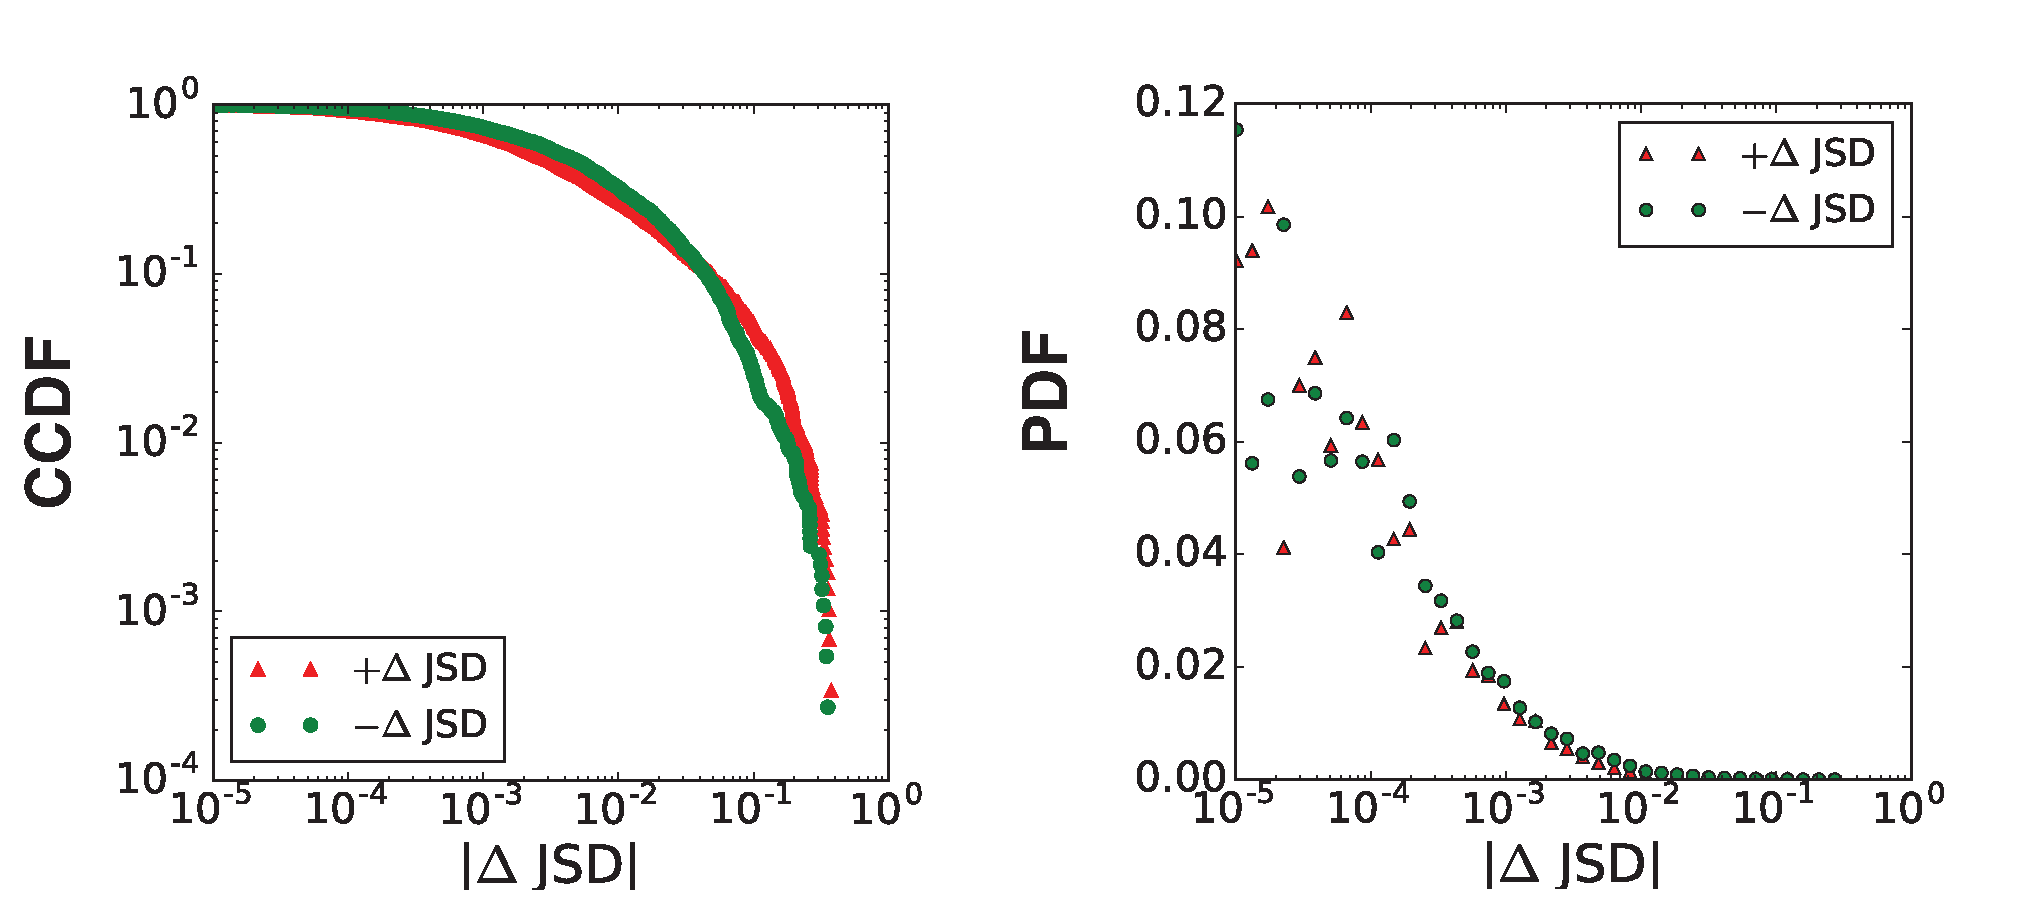
\includegraphics[width=15cm]{figures/distribution_JSD.eps}
\caption{jumps sizes}
\label{fig:jump_sizes_new}
\end{center}
\end{figure}

\begin{table}
  \centering 
  \begin{tabular}{|c|c|c|c|c|}
	\hline
% after \\ : \hline or \cline{col1-col2} \cline{col3-col4} ...
   treatment & exponent $\alpha_{-}$~&~$~p-value~$~& exponent $~\alpha_{+}~$ & $~p-value~$~\\
   \hline
  simple  & -1.13(5) & 0.000 &  -1.32(6) & 0.000\\
  complex &  -1.23(4) & 0.000 & -1.39(4) & 0.000\\
\hline
\end{tabular}
  \caption{Power law fits obtained by OLS regression of the log binned probability density function (come up with a better explanation or a better method). A comparison with log-normal is desirable because for the stochastic process formulation.}
  \label{pwlaw_fits}
\end{table}

\begin{figure}[h!]
\begin{center}
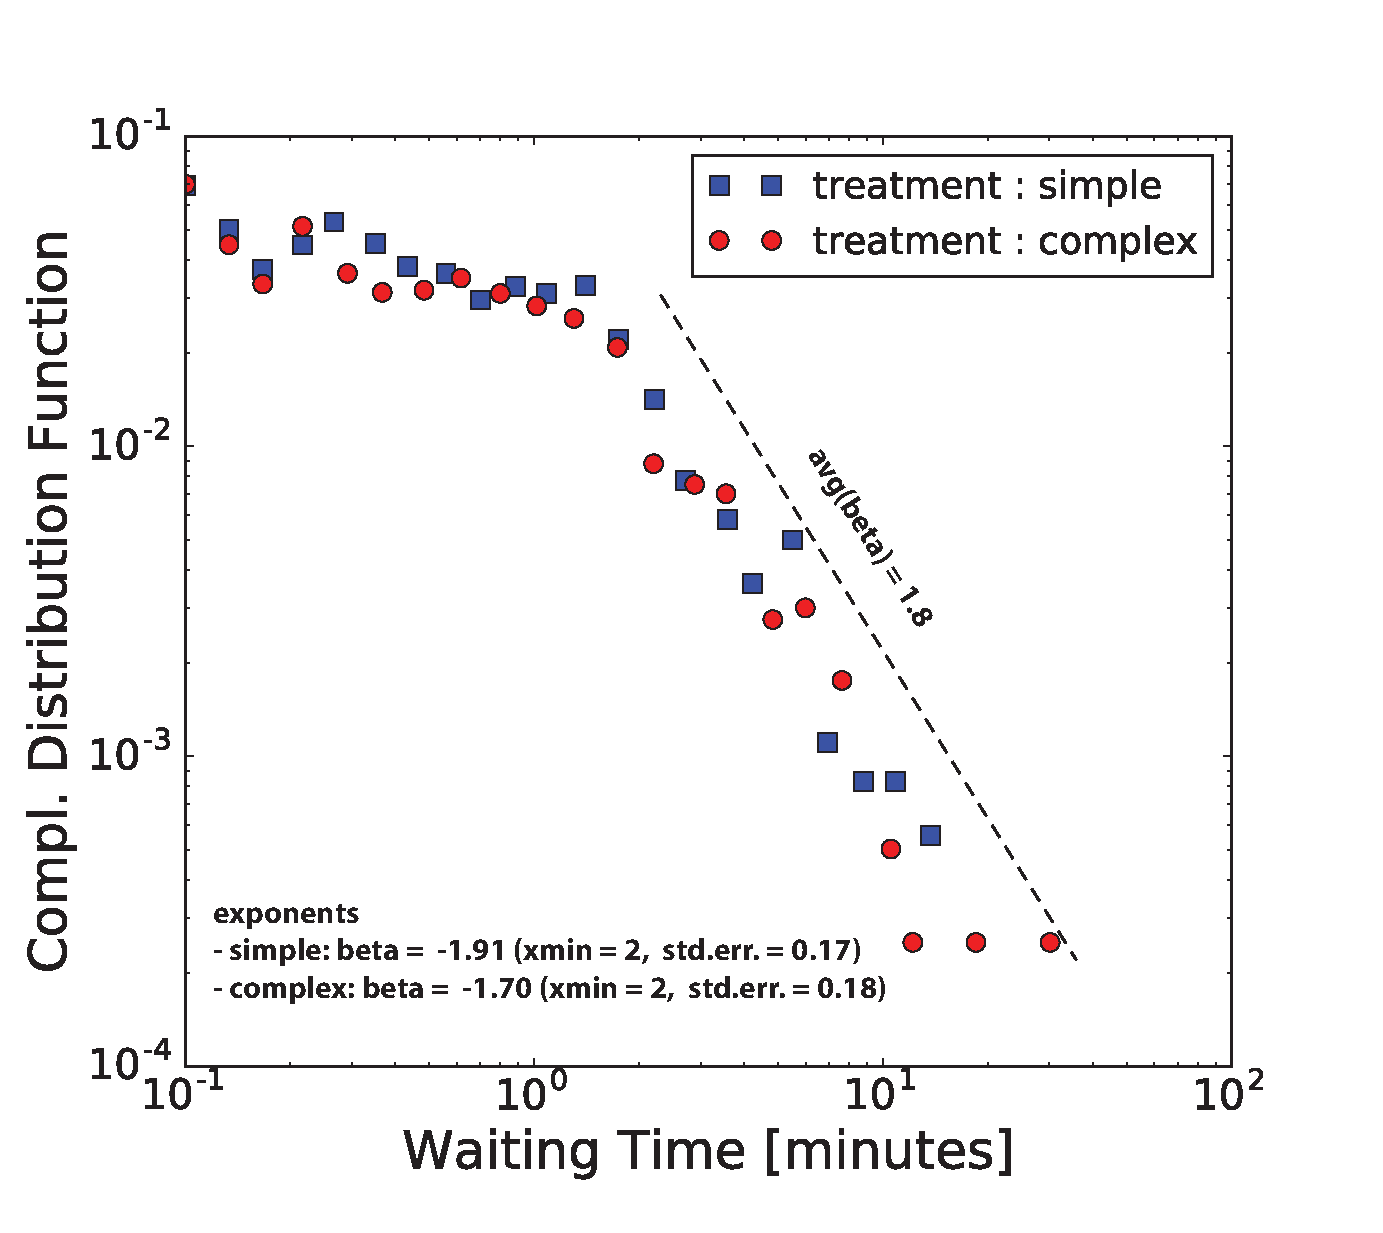
\includegraphics[width=15cm]{figures/ccdf_waiting_time.eps}
\caption{Distribution of Waiting Times is fairly the same in both the simple and complex cases.}
\label{fig:waiting_times}
\end{center}
\end{figure}

\begin{figure}[h!]
\begin{center}
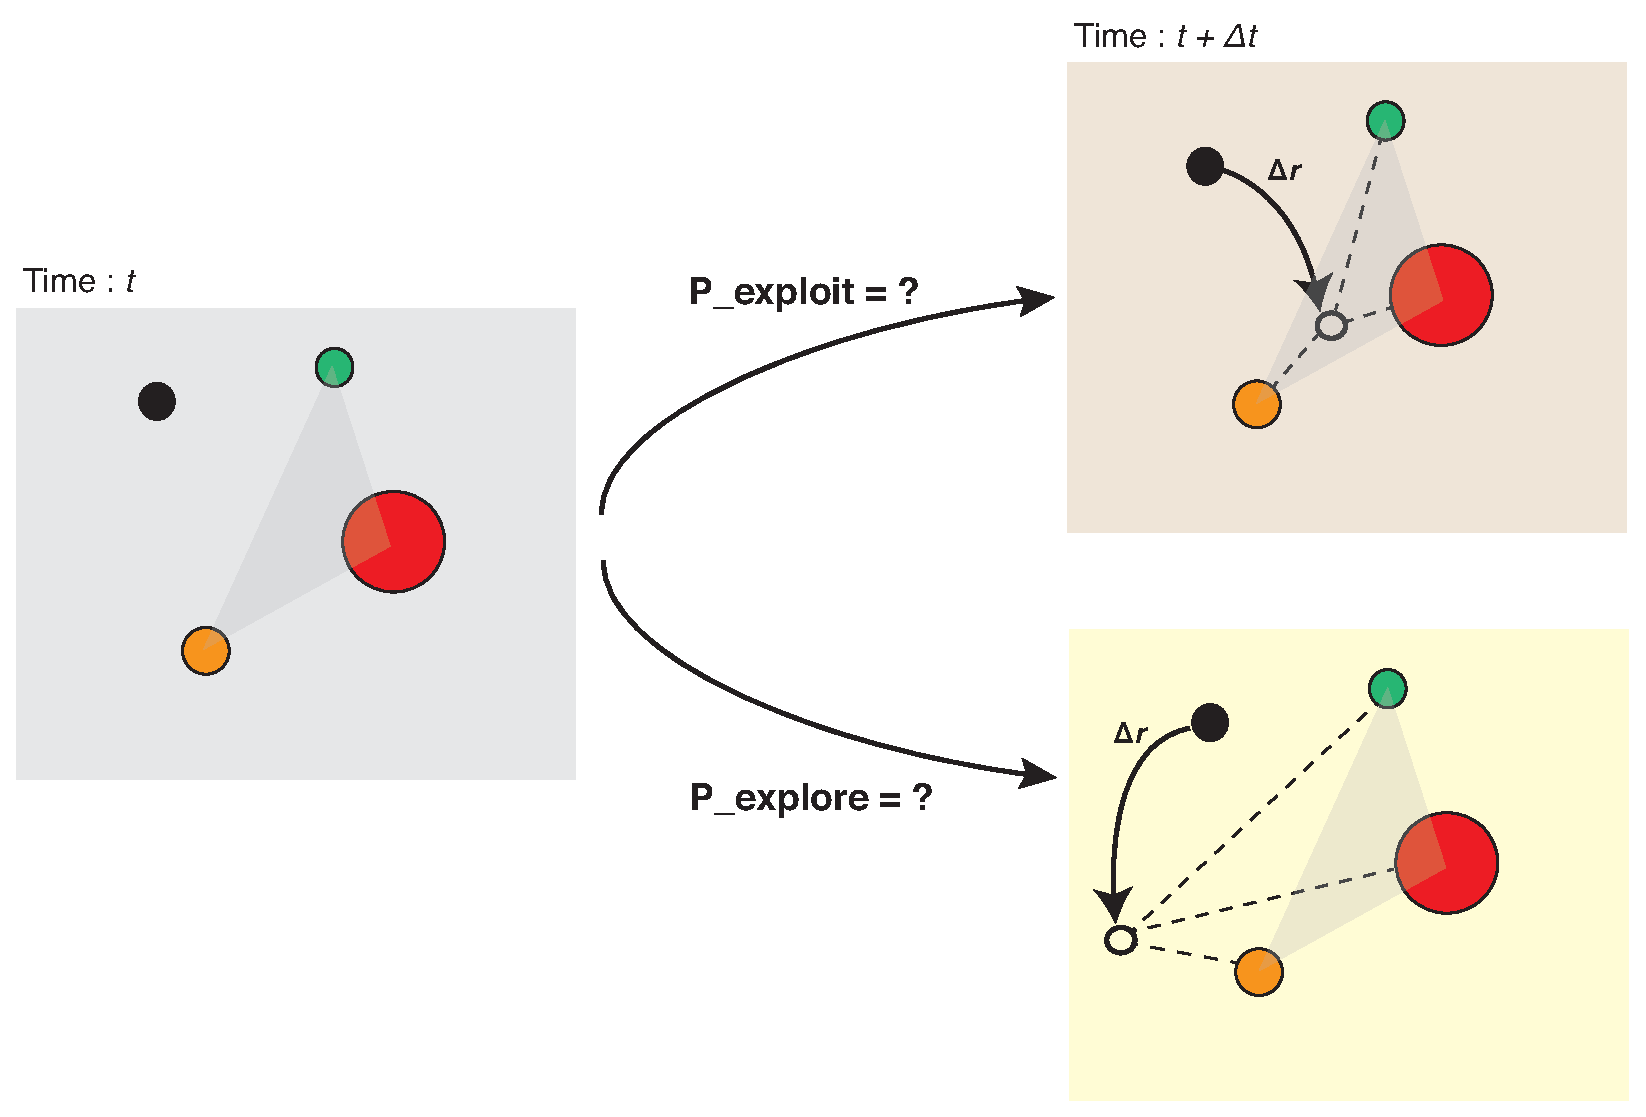
\includegraphics[width=15cm]{figures/schematic_displacement.eps}
\caption{2-dimensional schematic description of the {\it L\'evy flying mind} model ({\bf ``Proportional Attraction"}): At each time step, the individual must choose between remaining in the solution envelope that has already been explored and exploring outside the currently known solution envelope.  We assign some probability $p$ (a number between 0 and 1) to the participant's decision of staying in the explored envelop and probability $1-p$ to the decision to explore outside that envelop.  If it is harder to find solutions that offer a balanced re-combination of previous solutions than to think out-of-the-box and propose solutions outside of the current solution envelope, then $p < \frac{1}{2}$ else $p \geq \frac{1}{2}$.}
\label{fig:schematic}
\end{center}
\end{figure}

\begin{figure}[h!]
\begin{center}
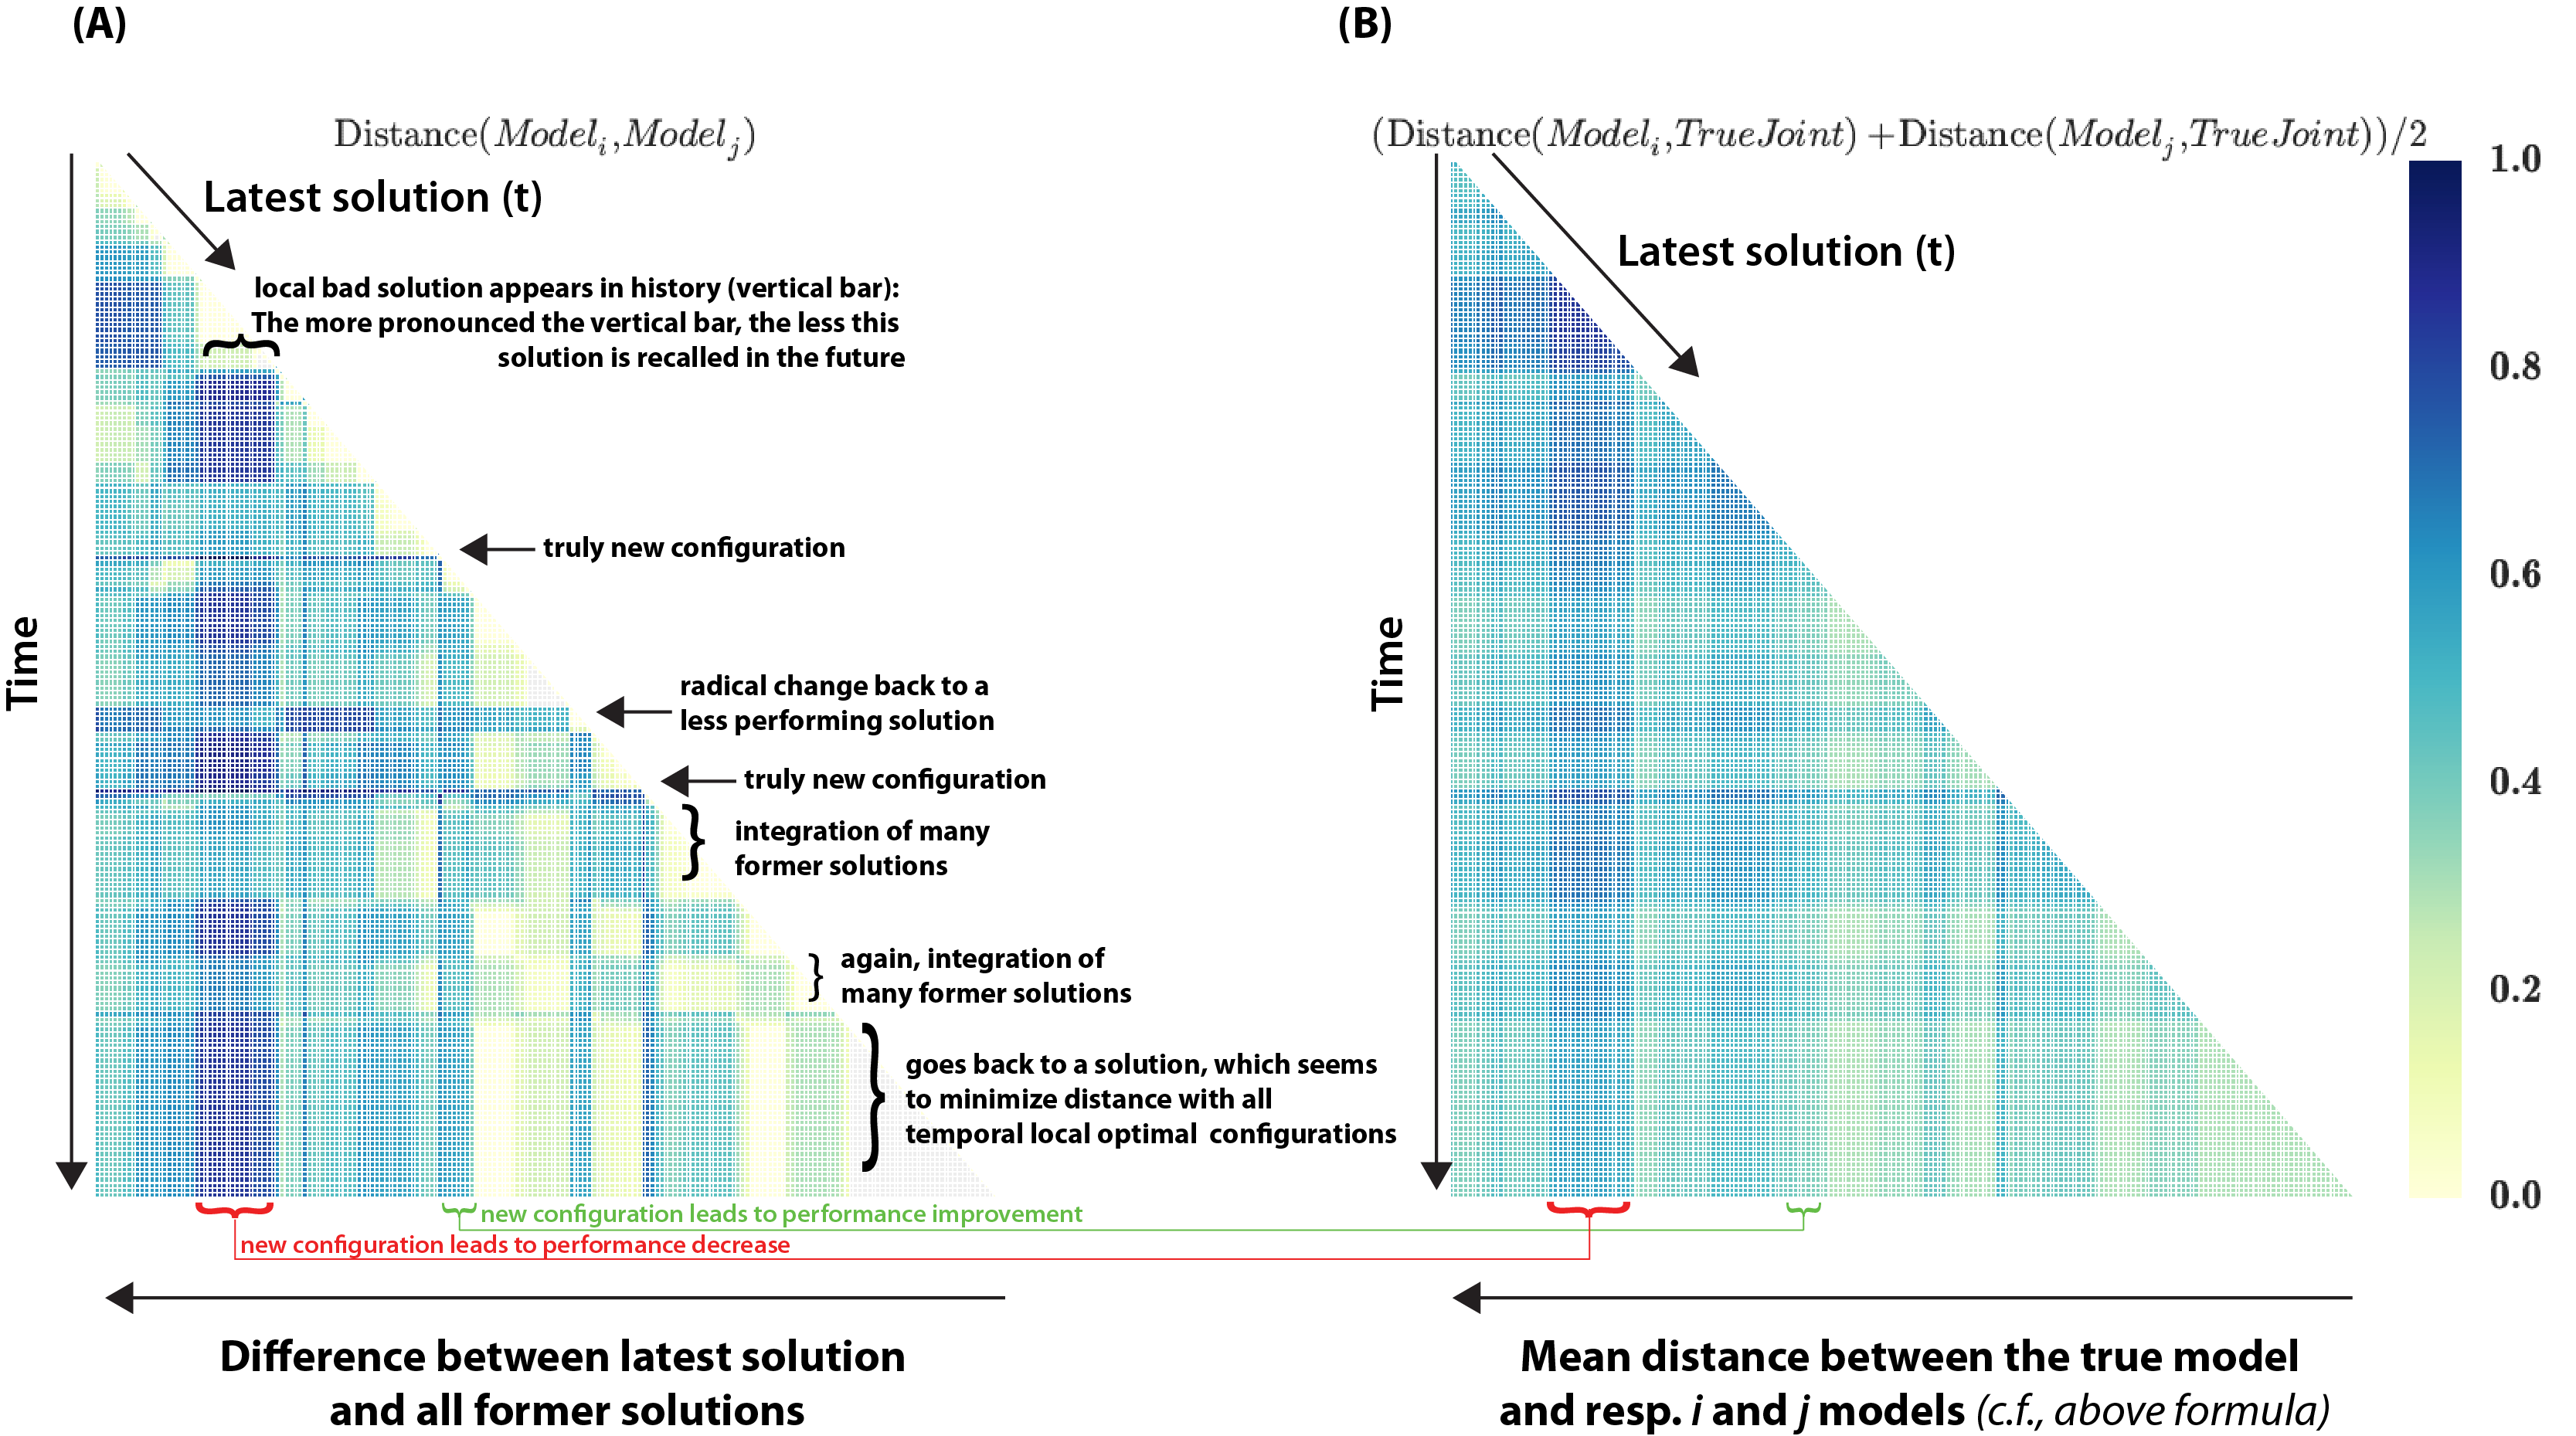
\includegraphics[width=15cm]{figures/matrice2.png}
\caption{\footnotesize The triangular matrix {\bf A} depicts the cognitive distances between a person's model at time $i$ and that same person's model at time $j$.  latest solution as a function of time and all former solutions, and {\bf B} of mean distance between the true model and resp. $i$ and $j$ configurations. Matrix {\bf B} shows the performance of a proposed model and serves as a reference for rationalizing choice sequences made by participants. These choice sequences are represented in matrix {\bf A} for participant 13: We see a wealth of characteristic choices leading to better of worse solutions, but also some integration and disruptive change in strategies, some which having a positive impact on performance, and other having a negative impact on performance. The rectangle structures show that participants do not drastically update drastically, but rather alternate periods of fine tuning and radical innovation. Matrix {\bf A} can also be watched in a more heuristic way at the coarse grained level: The more contrasted the pattern the more innovation overall. And, as shown here for participant 13, as more models are tested -- towards the lower right corner -- colors get more yellowish showing overall convergence of models. In the case presented here, the convergence of models leads overall to better solutions over time. It may not always be the case.}
\label{fig:matrices}
\end{center}
\end{figure}


\vspace{1cm}
\begin{figure}[h]
\label{init_final_best}
%\centerline{\epsfig{figure=../figures/histogram.eps,angle=0,width=14cm,scale=1}}
\caption{How does the initial guess influence the final (resp. best) score?}
\label{figure1}
\end{figure}

